\documentclass[../main.tex]{subfiles}

\begin{document}

\section{Átviteli függvények II}

\begin{fulltheorem}
  Adott két diszkrét idejű átviteli függvény ($W_1$ és $W_2$).
  Vezesse le az eredő átviteli függvény összefüggését, ha a két átviteli
  függvény sorba, párhuzamosan, illetve negatívan visszacsatolva kapcsolódik
  egymáshoz. Egyszerű példa kapcsán mutassa be, a hatásvázlat átalakításának
  szabályait a következő esetekben:
  \begin{itemize}
    \item Elágazási pont áthelyezése tag elől tag mögé
    \item Elágazási pont áthelyezése tag elé
    \item Összegzési pont áthelyezése tag mögé
    \item Összegzési pont áthelyezése tag elé
  \end{itemize}
\end{fulltheorem}

\subsection{Átviteli függvények sorba kapcsolása}

A sorosan kapcsolt átviteli függvények eredője az egyes átvitelek szorzata,
vagyis:
\[
  W_e(s) = \prod_{i=0}^n W_i(s)
\]

\begin{figure}[H]
  \centering
  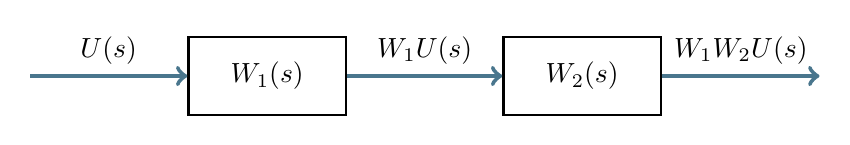
\begin{tikzpicture}[thick, arr/.style={ultra thick, draw=cyan!50!black}]
    \node[rectangle, minimum width=2cm, minimum  height=1cm, draw=black] (w1) at (0,0) {$W_1(s)$};
    \node[rectangle, minimum width=2cm, minimum  height=1cm, draw=black] (w2) at (4,0) {$W_2(s)$};

    \draw[to-, arr] (w1.west) -- ++(-2,0) node[midway, above] {$U(s)$};
    \draw[to-, arr] (w2) -- (w1) node[midway, above] {$W_1 U(s)$};
    \draw[-to, arr] (w2.east) -- ++(2,0) node[midway, above] {$W_1 W_2 U(s)$};
  \end{tikzpicture}
  \caption{Átviteli függvények sorba kapcsolása}
  \label{fig:linearW}
\end{figure}

\subsection{Átviteli függvények párhozamos kapcsolása}

A párhozamosan kapcsolt átviteli függvények eredője az egyes átvitelek összege,
vagyis:
\[
  W_e(s) = \sum_{i=0}^n W_i(s)
\]

\begin{figure}[H]
  \centering
  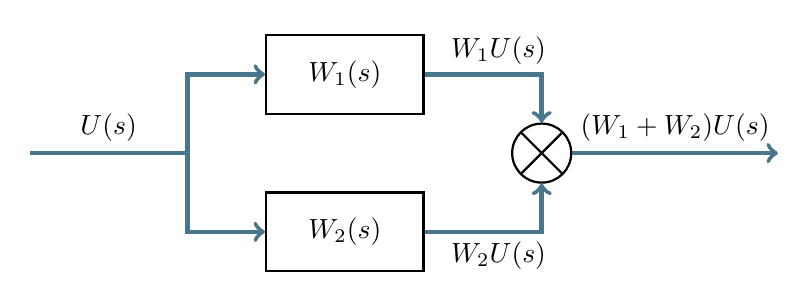
\begin{tikzpicture}[
      thick,
      arr/.style={ultra thick, draw=cyan!50!black},
      cross/.style={path picture={
              \draw[black]
              (path picture bounding box.south east) -- (path picture bounding box.north west) (path picture bounding
              box.south west)
              -- (path picture bounding box.north east);
            }}
    ]
    \node[rectangle, minimum width=2cm, minimum  height=1cm, draw=black] (w1) at (0,1) {$W_1(s)$};
    \node[rectangle, minimum width=2cm, minimum  height=1cm, draw=black] (w2) at (0,-1) {$W_2(s)$};
    \node[circle, minimum size=.75cm, draw=black, cross] (s) at (2.5,0) {};

    \draw[-to, arr] (-4,0) -- ++(2,0) node[midway, above] {$U(s)$} |- (w1);
    \draw[-to, arr] (-4,0) -- ++(2,0) |- (w2);
    \draw[-to, arr] (w1) -| (s) node[midway, above=3mm, left=-2mm] {$W_1 U(s)$};
    \draw[-to, arr] (w2) -| (s) node[midway, below=3mm, left=-2mm] {$W_2 U(s)$};
    \draw[-to, arr] (s) -- ++(3,0) node[midway, above] {$(W_1 + W_2) U(s)$};
  \end{tikzpicture}
  \caption{Átviteli függvények párhozamos kapcsolása}
  \label{fig:paralelW}
\end{figure}

\subsection{Visszacsatolás}

Visszacsatolás esetén az alábbiak alapján számítható az eredő átmeneti függvény:
\begin{gather*}
  Y(s) = W_1 U(s) \pm W_1 W_2 Y(s) \\
  (1 \mp W_1 W_2) Y(s) = W_1 U(s) \\
  W_e = \frac{Y(s)}{U(s)} = \frac{W_1}{1 \mp W_1 W_2}
\end{gather*}

\begin{figure}[H]
  \centering
  \begin{tikzpicture}[
      thick,
      arr/.style={ultra thick, draw=cyan!50!black},
      cross/.style={path picture={
              \draw[black]
              (path picture bounding box.south east) -- (path picture bounding box.north west) (path picture bounding
              box.south west)
              -- (path picture bounding box.north east);
            }}
    ]
    \node[rectangle, minimum width=2cm, minimum  height=1cm, draw=black] (w1) at (0,1) {$W_1(s)$};
    \node[rectangle, minimum width=2cm, minimum  height=1cm, draw=black] (w2) at (0,-1) {$W_2(s)$};
    \node[circle, minimum size=.75cm, draw=black, cross] (s) at (-2,1) {};

    \draw[to-, arr] (s) node[left=5mm, above=0mm] {$+$} -- ++(-2,0) node[midway, above] {$U(s)$};
    \draw[-to, arr] (s) -- (w1);
    \draw[-to, arr] (w1) -- ++(4,0) node[above left] {$\dfrac{W_1}{1 \mp W_1 W_2} U(s)$};
    \draw[-to, arr] ($(w1.east)+(1,0)$) |- (w2);
    \draw[-to, arr] (w2) -| (s) node[below=5mm, left=0mm] {$\pm$};
  \end{tikzpicture}
  \caption{Átviteli függvények párhozamos kapcsolása}
  \label{fig:boosterW}
\end{figure}

\subsection{Elágazási pont áthelyezése}

\begin{figure}[H]
  \centering
  \begin{tikzpicture}[
      thick,
      arr/.style={ultra thick, draw=cyan!50!black},
      box/.style={rectangle, minimum width=1.2cm, minimum  height=.75cm, draw=black, font=\scriptsize},
    ]
    \node[box] (w1) at (0,0) {$W_1(s)$};
    \node[box] (w2) at (0,-1.2) {$W_2(s)$};

    \draw[arr,to-] (w1) -- ++(-2.2,0);
    \draw[arr,to-] (w2) -| ++(-1.5,1.2);
    \draw[arr,-to] (w1) -- ++(2,0);
    \draw[arr,-to] (w2) -- ++(2,0);

    \draw[gray, dash pattern=on 2.25mm off .75mm, -to, very thick] ($(w1)-(1.5,0)$) to[bend left=60] ++(3,0);

    \begin{scope}[xshift=5cm]
      \node[box] (w11) at (0,0) {$W_1(s)$};
      \node[box] (w12) at (2.5,-1.2) {$1 / W_1(s)$};
      \node[box] (w2) at (4.5,-1.2) {$W_2(s)$};

      \draw[arr,to-] (w11) -- ++(-1.5,0);
      \draw[arr,to-] (w12) -| ++(-1.2,1.2);
      \draw[arr,-to] (w11) -- ++(6,0);
      \draw[arr,-to] (w12) -- (w2);
      \draw[arr,-to] (w2) -- ++(1.5,0);
    \end{scope}
  \end{tikzpicture}
  \caption{Elágazási pont áthelyezése a tag mögé}
  \label{fig:dotforwardW}
\end{figure}

\begin{figure}[H]
  \centering
  \begin{tikzpicture}[
      thick,
      arr/.style={ultra thick, draw=cyan!50!black},
      box/.style={rectangle, minimum width=1.2cm, minimum  height=.75cm, draw=black, font=\scriptsize},
    ]
    \node[box] (w) at (0,0) {$W(s)$};

    \draw[arr,to-] (w) -- ++(-2.2,0);
    \draw[arr,-to] (w) -- ++(2.2,0);
    \draw[arr,-to] ($(w)+(1.2,0)$) |- ++(1,-1.2);

    \draw[gray, dash pattern=on 2.25mm off .75mm, to-, very thick] ($(w1)-(1.5,0)$) to[bend left=60] ++(2.7,0);

    \begin{scope}[xshift=6cm]
      \node[box] (w1) at (0,0) {$W(s)$};
      \node[box] (w2) at (0,-1.2) {$W(s)$};

      \draw[arr,to-] (w1) -- ++(-2.2,0);
      \draw[arr,to-] (w2) -| ++(-1.5,1.2);
      \draw[arr,-to] (w1) -- ++(1.5,0);
      \draw[arr,-to] (w2) -- ++(1.5,0);
    \end{scope}
  \end{tikzpicture}
  \caption{Elágazási pont áthelyezése a tag elé}
  \label{fig:dotbackwardW}
\end{figure}

\subsection{Összegzési pont áthelyezése}

\begin{figure}[H]
  \centering
  \begin{tikzpicture}[
      thick,
      arr/.style={ultra thick, draw=cyan!50!black},
      box/.style={rectangle, minimum width=1.2cm, minimum  height=.75cm, draw=black, font=\scriptsize},
      cross/.style={path picture={
              \draw[black]
              (path picture bounding box.south east) -- (path picture bounding box.north west) (path picture bounding
              box.south west)
              -- (path picture bounding box.north east);
            }}
    ]
    \node[circle, minimum size=.75cm, draw=black, cross] (s) at (0,0) {};
    \node[box] (w) at (2,0) {$W(s)$};

    \draw[arr,to-] (s) -- ++(-1.5,0);
    \draw[arr,to-] (s) |- ++(-1.5,-1.2);
    \draw[arr,-to] (s) -- (w);
    \draw[arr,-to] (w) -- ++(1.8,0);

    \draw[gray, dash pattern=on 2.25mm off .75mm, -to, very thick] (s) to[bend left=60] ($(w)+(1.2,0)$);

    \begin{scope}[xshift=7cm]
      \node[box] (w1) at (0,0) {$W(s)$};
      \node[box] (w2) at (0,-1.2) {$W(s)$};
      \node[circle, minimum size=.75cm, draw=black, cross] (s) at (2,0) {};


      \draw[arr,-to] (s) -- ++(1.2,0);
      \draw[arr,-to] (w1) -- (s);
      \draw[arr,-to] (w2) -| (s);
      \draw[arr,to-] (w1) -- ++(-1.8,0);
      \draw[arr,to-] (w2) -- ++(-1.8,0);
    \end{scope}
  \end{tikzpicture}
  \caption{Összegzési pont áthelyezése a tag mögé}
  \label{fig:sumforwardW}
\end{figure}

\begin{figure}[H]
  \centering
  \begin{tikzpicture}[
      thick,
      arr/.style={ultra thick, draw=cyan!50!black},
      box/.style={rectangle, minimum width=1.2cm, minimum  height=.75cm, draw=black, font=\scriptsize},
      cross/.style={path picture={
              \draw[black]
              (path picture bounding box.south east) -- (path picture bounding box.north west) (path picture bounding
              box.south west)
              -- (path picture bounding box.north east);
            }}
    ]
    \node[box] (w) at (0,0) {$W(s)$};
    \node[circle, minimum size=.75cm, draw=black, cross] (s) at (2,0) {};

    \draw[arr,to-] (w) -- ++(-1.8,0);
    \draw[arr,-to] (w) -- (s);
    \draw[arr,-to] (s) -- ++(1.2,0);
    \draw[arr,to-] (s) |- ++(-3.8,-1.2);

    \draw[gray, dash pattern=on 2.25mm off .75mm, -to, very thick] (s) to[bend right=60] ($(w)-(1.2,0)$);

    \begin{scope}[xshift=8cm]
      \node[circle, minimum size=.75cm, draw=black, cross] (s) at (0,0) {};
      \node[box] (w1) at (2,0) {$W(s)$};
      \node[box] (w2) at (-1.5,-1.2) {$1/W(s)$};

      \draw[arr,-to] (w1) -- ++(1.3,0);
      \draw[arr,-to] (s) -- (w1);
      \draw[arr,to-] (s) -- ++(-3.3,0);
      \draw[arr,to-] (w2) -- ++(-1.8,0);
      \draw[arr,-to] (w2) -| (s);
    \end{scope}
  \end{tikzpicture}
  \caption{Összegzési pont áthelyezése a tag elé}
  \label{fig:sumbackwardW}
\end{figure}

\end{document}
